%!TEX TX-program = xelatex
\documentclass[8pt]{article}

\usepackage{ctex}
\usepackage{graphicx}
\usepackage{enumitem}
\usepackage{geometry}
\usepackage{amsmath}
\usepackage{amssymb}
\usepackage{amsfonts}
\usepackage{tikz}
\usepackage{extarrows}
\usetikzlibrary{positioning}
\usepackage{xcolor}

\graphicspath{ {./images/} }

\title{1 集合}
\author{高一(6)班\ 邵亦成\ 26号}

\geometry{a4paper, scale=0.8}

\setcounter{section}{0}

\begin{document}

	\maketitle

	\section{集合}
		\subsection{集合初步}
			\subsubsection{集合的关系}
				\textbf{集合:}一些确定对象的全体.

				\textbf{集合中元素的特征:}确定性,互异性,无序性.

				\textbf{集合符号}:大写字母$A, B, C, \dots$.

				\textbf{元素符号}:小写字母$a, b, c, \dots$.

				\textbf{二元逻辑符号}:元素$a$在集合$S$中:$a\in S$;元素$a$不在集合$S$中:$a\notin S$;集合$A$与集合$B$相同:$A=B$;集合$A$与集合$B$不同:$A\neq B$.

				\textbf{集合的分类}:空集,有限集,无限集.

				\textbf{空集}:不含任何元素的集合,记作$\emptyset$.

				\textbf{全集}:所有研究对象组成的集合,用符号$U$来表示.

				\textbf{特殊数集}:有理数集$\mathbf{N}$,正整数集$\mathbf{N}^{*}$,整数集$\mathbf{Z}$,有理数集$\mathbf{Q}$,实数集$\mathbf{R}$. 在$\mathbf{Z}, \mathbf{Q}, \mathbf{R}$后加一上标$+$或$-$表示对应的正数/负数集合.

				\textbf{集合表示形式}:列举法、描述法、图示法.

				\textbf{列举法}:$A=\left\{a,b,c,\dots\right\}.$

				\textbf{描述法}:$A=\left\{x|x\text{满足性质}p\right\}.$表示$A$为所有满足性质$p$的$x$组成的集合.

				\textbf{图示法}:即文氏图法.

				$$
					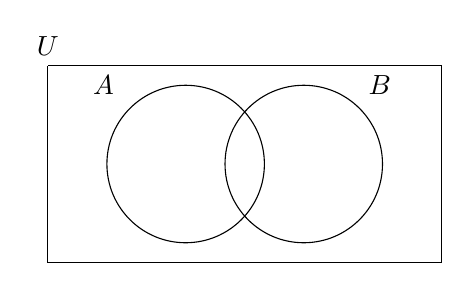
\begin{tikzpicture} [scale=0.25]
						\draw [black] (-10,  5)--( 10,  5)--( 10, -5)--(-10, -5)--(-10,  5) node[anchor=south] {$U$};

						\draw [black] (-3, 0) circle (4); 

						\node [text width=1em] at (-7, 4) {$A$};

						\draw [black] ( 3, 0) circle (4);

						\node [text width=1em] at ( 7, 4) {$B$};


					\end{tikzpicture}
				$$

				\textbf{子集}:对$A$中的任意元素$x$都有$x\in B$,记作$A\subseteq B$或$B\supseteq A$. 规定$\emptyset \subseteq A$,其中$A$为任意集合.

				\textbf{真子集}:对$A$中的任意元素$x$都有$x\in B$,且$A\neq B$,记作$A\subset B$或$B\supset A$. 规定$\emptyset \subset A$,其中$A$为任意非空集合.

				\textbf{(真)子集的性质}:(真)子集同大于/小于号,具有相同方向的传递性;$A=B$当且仅当$A\subseteq B$且$B\subseteq A$.

				\textbf{子集的个数}:若$|S|=n$,则$\displaystyle\sum_{A\subseteq S} 1=2^n, \sum_{A\subset S} 1=2^n-1.$

				\textbf{空集的连接符号}:$\emptyset \in \{\emptyset\}, \emptyset \subseteq \{\emptyset\}, \emptyset \subset \{\emptyset\}, \emptyset \neq \{\emptyset\}.$

				\textbf{区间}:$[a,b]=\{x|a\leq x\leq b\}, (a,b)=\{x|a<x<b\} (a<b)$,半开半闭区间同理,一侧为$\pm\infty$即表示无该端点限制.

				~\\

				\textbf{例一}:已知:$A=\left\{x|x=2n+1, n\in\mathbf{Z}\right\}, B=\left\{x|x=2n-1, n\in\mathbf{Z}\right\}$. 求证:$A=B$.
				~\\

				\begin{enumerate}[label=$\arabic*^{\circ}$]
					\item 证明$A\subseteq B$

						$\forall x\in A: x=2n+1=2(n+1)-1.$

						$\because n\in\mathbf{Z}\therefore n+1\in\mathbf{Z}.$

						$\therefore x\in B \therefore A\subseteq B.$

					\item 证明$B\subseteq A$

						$\forall x\in B: x=2n-1=2(n-1)+1.$

						$\because n\in\mathbf{Z}\therefore n-1\in\mathbf{Z}.$

						$\therefore x\in A \therefore B\subseteq A.$

				\end{enumerate}

				综上,$A=B$.

				\textcolor{red}{\textbf{总结:证明$A=B$可以使用$A\subseteq B$且$B\subseteq A$,两者等价.}}
				
				~\\

				\textbf{例二}:已知:$A=\{x,x^2,xy\}, B=\{1,x,y\}, A=B$. 求:$x,y$.
				~\\

				分两种对应情况讨论.

				\begin{enumerate}[label=$\arabic*^{\circ}$]

					\item $\displaystyle \left\{\begin{array}{rcl}xy&=&y\\x^2&=&1\end{array}\right.$

						$\because x\neq x^2 \therefore x=-1.$

						$\because xy=y \therefore y=0.$

					\item $\displaystyle \left\{\begin{array}{rcl}xy&=&1\\x^2&=&y\end{array}\right.$

						解得$x=1$(舍).

				\end{enumerate}

				综上,$x=-1, y=0$.

				\textcolor{red}{\textbf{总结:求解$A=B$使用对应元素相等分类讨论列方程并通过集合元素的互异性进行检验.}}

				~\\

				\textbf{例三}:已知:$A=\{x,xy,x+y\}, B=\{0,|x|,y\}, A=B$. 求:$A$.
				~\\

				$\because B=\{0,|x|,y\}$

				$\therefore |x|\neq 0, y\neq 0$

				$\therefore x\neq 0, xy\neq 0$

				$\therefore x+y\neq 0.$

				分两种对应情况讨论.

				\begin{enumerate}[label=$\arabic*^{\circ}$]

					\item $\displaystyle \left\{\begin{array}{rcl}x&=&|x|\\xy&=&y\end{array}\right. \Rightarrow \left\{\begin{array}{rcl}x&=&1\\y&=&-1\end{array}\right.$

						此时$A=\{1, -1, 0\}, B=\{0, 1, -1\}$,符合.

					\item $\displaystyle \left\{\begin{array}{rcl}xy&=&|x|\\x&=&y\end{array}\right. \overset{|x|^2=x^2}{\Longrightarrow} \left\{\begin{array}{rcl}x&=&1\\y&=&1\end{array}\right.$

						此时$A=\{1, 1, 2\}$(舍).

				\end{enumerate}

				综上,$A=\{1, -1, 0\}.$

				\textcolor{red}{\textbf{总结:求解$A=B$对应形式若过多可使用互异性等首先排除部分对应条件后进行讨论.}}

				~\\

				\textbf{例四}:已知:$M=\{x|ax+1=0\}, N=\{x|x^2-5x+6=0\}, M\subset N$.求:$a$.
				~\\

				$N=\{2,3\}.$

				分两类讨论.

				\begin{enumerate}[label=$\arabic*^{\circ}$]

					\item $M=\emptyset$
						即$ax+1=0$无解$\Rightarrow a=0.$

					\item $M\neq \emptyset$即$a\neq 0$

						$ax+1=0$的根为$x=-\frac{1}{a}.$

						$\because M\subset N$

						$\therefore -\frac{1}{a}=2 \text{ or } -\frac{1}{a}=3$

						$\therefore a=-\frac{1}{2} \text{ or } -\frac{1}{3}.$

				\end{enumerate}

				综上,$a\in\left\{0, -\frac{1}{2}, -\frac{1}{3}\right\}$

				\textcolor{red}{\textbf{总结:$A\subset B$及$A\subseteq B$类题勿忘考虑$A=\emptyset$.}}

				~\\

				\textbf{例五}:已知:$A=\{x|-3\leq x\leq 4\}, B=\{x|2m-1\leq x\leq m+1\}, B\subseteq A.$ 求:$m$.
				~\\

				分两类讨论.

				\begin{enumerate}[label=$\arabic*^{\circ}$]

					\item $B=\emptyset$

						即$2m-1>m+1 \Rightarrow m>2$.

					\item $B\neq\emptyset \Rightarrow m\leq 2$

						$\displaystyle \left\{\begin{array}{rcl}2m-1&\geq&3\\m+1&\leq&4\end{array}\right. \Rightarrow m\in[-1,3].$

						$\because m\leq 2$

						$\therefore m\in[-1, 2].$

				\end{enumerate}

				综上,$m\geq -1$.

				\textcolor{red}{\textbf{总结:分类讨论每个类的结论都应该在这个类的大前提之下.}}

				~\\

				\textbf{例六}:已知:$S\subset \mathbf{N}, S\neq \emptyset, \forall x\in S: 1+\frac{11}{x-1}\in S.$

				\begin{enumerate}[label=$(\arabic*)$]

					\item $S$能否为单元素集?为什么?
					\item 求出只含两个元素的集合$S$.
					\item 满足条件的$S$一共有几个?为什么?并列举它们.

				\end{enumerate}

				\begin{enumerate}[label=$(\arabic*)$]

					\item $S$能否为单元素集?为什么?

						$\because \forall x\in S: 1+\frac{11}{x-1}\in S$

						$\therefore$若$S$为单元素集,则有$x\in\mathbf{N}$且$x=1+\frac{12}{x-1}$

						解得$x=1\pm 2\frac{3} \notin \mathbf{N}.$

						$\therefore S$不能为单元素集.

					\item 求出只含两个元素的集合$S$.

						$\because x\in\mathbf{N}, 1+\frac{12}{x-1}\in\mathbf{N}$

						$\therefore x-1\in\{1,2,3,4,6,12\}$即$x$可取$2,3,4,5,7,13.$

						$x=2 \Rightarrow 1+\frac{12}{x-1}=13.$

						$x=13 \Rightarrow 1+\frac{12}{x-1}=2.$

						$x=3 \Rightarrow 1+\frac{12}{x-1}=7.$

						$x=7 \Rightarrow 1+\frac{12}{x-1}=3.$

						$x=4 \Rightarrow 1+\frac{12}{x-1}=5.$

						$x=5 \Rightarrow 1+\frac{12}{x-1}=4.$

						即$S=\{2,13\}\text{ or }\{3,7\}\text{ or }\{4,5\}.$

					\item 满足条件的$S$一共有几个?为什么?并列举它们.

						$2^3-1=7.$

						$\{2,13\}, \{3,7\}, \{4,5\}, \{2,3,7,13\}, \{2,4,5,13\}, \{3,4,5,7\}, \{2,3,4,5,7,13\}.$
				
				\end{enumerate}

				\textcolor{red}{\textbf{总结:突破口在于$S\subset N$,随后根据条件中的分式考虑分子的因数代入计算检验.}}

				~\\

				\textbf{例七}:已知:$A=\{x|0<ax+1\leq 5\}, B=\{x|\frac{1}{2}<x\leq 2\}.$

				\begin{enumerate}[label=$(\arabic*)$]

					\item 若$A\subseteq B$,求$a$.
					\item 若$A\supseteq B$,求$a$.
					\item $A, B$能否相等?求出$a$并说明理由.

				\end{enumerate}

				\begin{enumerate}[label=$\arabic*^{\circ}$]
					\item $a=0\Rightarrow 0<1\leq 5 \Rightarrow A=\mathbf{R}.$
					\item $a>0\Rightarrow A=\left(-\frac{1}{a}, \frac{4}{a}\right].$
					\item $a<0\Rightarrow A=\left[\frac{4}{a}, -\frac{1}{a}\right).$
				\end{enumerate}
				\begin{enumerate}[label=$(\arabic*)$]

					\item 若$A\subseteq B$,求$a$.

						$\because A\subseteq B$

						$\therefore$分两类讨论.

						\begin{enumerate}[label=$\arabic*^{\circ}$]
							\item $a>0$
								$$
									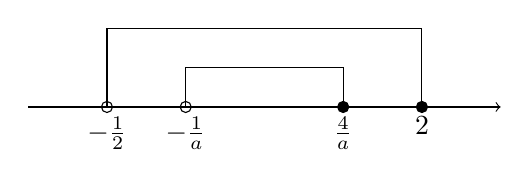
\begin{tikzpicture} [scale=0.5]
										\draw [black] [->] (-6, 0)--(6, 0);
										\draw [black] (-4, 0) circle (4pt) node[anchor=north] {$-\frac{1}{2}$};
										\filldraw [black] (4, 0) circle (4pt) node[anchor=north] {$2$};
										\draw [black] (-2, 0) circle (4pt) node[anchor=north] {$-\frac{1}{a}$};
										\filldraw [black] (2, 0) circle (4pt) node[anchor=north] {$\frac{4}{a}$};
										\draw [black] (-4, 0)--(-4, 2)--(4, 2)--(4, 0);
										\draw [black] (-2, 0)--(-2, 1)--(2, 1)--(2, 0);
									\end{tikzpicture}
								$$
								$\displaystyle\left\{\begin{array}{rcl}-\frac{1}{2}&\leq&-\frac{1}{a}\\\frac{4}{a}&\leq&2\end{array}\right.\Rightarrow a\geq 2.$

							\item $a<0$
								$$
									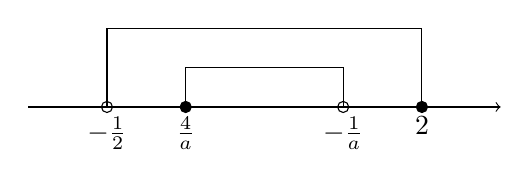
\begin{tikzpicture} [scale=0.5]
										\draw [black] [->] (-6, 0)--(6, 0);
										\draw [black] (-4, 0) circle (4pt) node[anchor=north] {$-\frac{1}{2}$};
										\filldraw [black] (4, 0) circle (4pt) node[anchor=north] {$2$};
										\filldraw [black] (-2, 0) circle (4pt) node[anchor=north] {$\frac{4}{a}$};
										\draw [black] (2, 0) circle (4pt) node[anchor=north] {$-\frac{1}{a}$};
										\draw [black] (-4, 0)--(-4, 2)--(4, 2)--(4, 0);
										\draw [black] (-2, 0)--(-2, 1)--(2, 1)--(2, 0);
									\end{tikzpicture}
								$$
								$\displaystyle\left\{\begin{array}{rcl}-\frac{1}{2}&<&\frac{4}{a}\\-\frac{1}{a}&\leq&2\end{array}\right.\Rightarrow a<-8.$
						\end{enumerate}

						综上,$a\in(-\infty, -8)\cup[2, +\infty).$

					\item 若$A\supseteq B$,求$a$.

						$\because A\supseteq B$

						$\therefore$分三类讨论.

						\begin{enumerate}[label=$\arabic*^{\circ}$]
							\item $a=0\Rightarrow A=\mathbf{R}\supseteq B$符合题意.

							\item $a>0$
								$$
									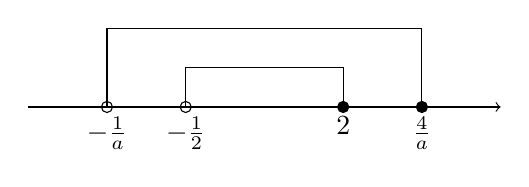
\begin{tikzpicture} [scale=0.5]
										\draw [black] [->] (-6, 0)--(6, 0);
										\draw [black] (-4, 0) circle (4pt) node[anchor=north] {$-\frac{1}{a}$};
										\filldraw [black] (4, 0) circle (4pt) node[anchor=north] {$\frac{4}{a}$};
										\draw [black] (-2, 0) circle (4pt) node[anchor=north] {$-\frac{1}{2}$};
										\filldraw [black] (2, 0) circle (4pt) node[anchor=north] {$2$};
										\draw [black] (-4, 0)--(-4, 2)--(4, 2)--(4, 0);
										\draw [black] (-2, 0)--(-2, 1)--(2, 1)--(2, 0);
									\end{tikzpicture}
								$$
								$\displaystyle\left\{\begin{array}{rcl}2&\leq&\frac{4}{a}\\-\frac{1}{a}&\leq&-\frac{1}{2}\end{array}\right.\Rightarrow 0<a\leq2.$

							\item $a<0$
								$$
									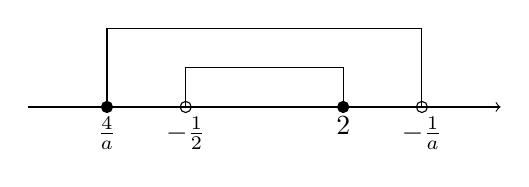
\begin{tikzpicture} [scale=0.5]
										\draw [black] [->] (-6, 0)--(6, 0);
										\draw [black] (-2, 0) circle (4pt) node[anchor=north] {$-\frac{1}{2}$};
										\filldraw [black] (2, 0) circle (4pt) node[anchor=north] {$2$};
										\filldraw [black] (-4, 0) circle (4pt) node[anchor=north] {$\frac{4}{a}$};
										\draw [black] (4, 0) circle (4pt) node[anchor=north] {$-\frac{1}{a}$};
										\draw [black] (-4, 0)--(-4, 2)--(4, 2)--(4, 0);
										\draw [black] (-2, 0)--(-2, 1)--(2, 1)--(2, 0);
									\end{tikzpicture}
								$$
								$\displaystyle\left\{\begin{array}{rcl}-\frac{1}{a}&>&2\\\frac{4}{a}&\leq&-\frac{1}{2}\end{array}\right.\Rightarrow -\frac{1}{2}<a<0.$
						\end{enumerate}

						综上,$a\in\left(-\frac{1}{2}, 2\right].$

					\item $A, B$能否相等?求出$a$并说明理由.

						能. 即$A\subseteq B, B\subseteq A$

						即$a\in((-\infty, -8)\cup[2, +\infty))\cap\left(-\frac{1}{2}, 2\right]$

						即$a=2.$

				\end{enumerate}

				\textcolor{red}{\textbf{总结:区间的子集的分析可借助数轴,注意空心点与实心点的区别及端点是否能取到问题.}}

			\subsubsection{集合的运算(交集、并集)}

				\textbf{交集}:集合$A$与集合$B$的交集为所有在集合$A$中\textbf{且}在集合$B$中的元素组成的集合. 记作$A\cap B=\{x|x\in A\textbf{ and }x\in B\}.$

				\textbf{并集}:集合$A$与集合$B$的并集为所有在集合$A$中\textbf{或}在集合$B$中的元素组成的集合. 记作$A\cup B=\{x|x\in A\textbf{ or }x\in B\}.$

				\textbf{交换律}:$A\cap B=B\cap A$;$A\cup B=B\cup A$.

				\textbf{结合律}:$A\cap (B\cap C) = (A\cap B)\cap C$;$A\cup (B\cup C) = (A\cup B)\cup C$.

				\textbf{分配律}:$A\cap(B\cup C)=(A\cap B)\cup(A\cap C)$;$A\cup(B\cap C)=(A\cup B)\cap(A\cup C)$.

				\textbf{同一律}:$A\cup\emptyset=A$;$A\cap U=A$.

				\textbf{零一律}:$A\cup U=U$;$A\cap\emptyset=\emptyset$.

				\textbf{等幂律}:$A\cup A=A$;$A\cap A=A$.

				\textbf{子集与交、并运算的关系}:$A\subseteq B\Leftrightarrow A\cup B=B \Leftrightarrow A\cap B=A$.

				\textbf{吸收律}:$A\cup(A\cap B)=A$;$A\cap(A\cup B)=A$.

				~\\

				\textbf{例一}:

				\begin{enumerate}[label=(\arabic*)]
					\item 已知:$A=\{y|y=x^2-2x+3, x\in\mathbf{R}\}, B=\{y|y=-x^2+2x+10,x\in\mathbf{R}\}.$ 求:$A\cap B$.

						$A=[2, +\infty), B=(-\infty, 11] \Rightarrow A\cap B=[2, 11].$

					\item 已知:$A=\{(x,y)|y=x+1, x\in\mathbf{R}\}, B=\{(x,y)|y=-x^2+2x+\frac{3}{4},x\in\mathbf{R}\}.$ 求:$A\cap B$.

						$\displaystyle x+1=-x^2+2x+\frac{3}{4} \Rightarrow x^2-x+\frac{1}{4}=0 \Rightarrow x=\frac{1}{2} \Rightarrow A\cap B=\left\{\left(\frac{1}{2}, \frac{3}{2}\right)\right\}.$
				\end{enumerate}

				\textcolor{red}{\textbf{总结:注意集合的元素类型是数还是点,以及数/点的实际含义.}}

				~\\

				\textbf{例二}:已知:$A=\{x|-2\leq x\leq4\}, B=\{x|x>a\}.$

				\begin{enumerate}[label=(\arabic*)]
					\item 若$A\cap B\neq\emptyset$,求:$a$.

					\item 若$A\cap B\neq A$,求:$a$.
				\end{enumerate}

				\begin{enumerate}[label=(\arabic*)]
					\item 若$A\cap B\neq\emptyset$,求$a$.

						考虑$A\cap B=\emptyset$有$a\geq 4$.

						于是$a<4$.

					\item 若$A\cap B\neq A$,求$a$.

						考虑$A\cap B=A$即$A\subseteq B$有$a<-2$.

						于是$A\cap B\neq A$时,$a\geq -2$.

				\end{enumerate}

				\textcolor{red}{\textbf{总结:考虑一个问题比较复杂时,可以考虑它的反面(补集运算的排中律).}}

				~\\

				\textbf{例三}:已知:$A=\{x|x^2+4x=0\}, B=\{x|x^2+2(a+1)x+a^2-1=0\}.$

				\begin{enumerate}[label=(\arabic*)]
					\item 若$A\cap B=B$,求:$a$.

					\item 若$A\cup B=B$,求:$a$.
				\end{enumerate}

				\begin{enumerate}[label=(\arabic*)]
					\item 若$A\cap B=B$,求:$a$.

						即$B\subseteq A$,分两类讨论:

						\begin{enumerate}[label=$\arabic*^{\circ}$]

							\item $B=\emptyset$

								有$x^2+2(a+1)x+a^2-1=0$无解,

								$\displaystyle\begin{array}{rcl}\therefore\ \Delta&=&4(a+1)^2-4a^2+4\\&=&8a+8\\&<&0\end{array}$

								$\Rightarrow a<-1.$

							\item $B\neq\emptyset$,即$a\geq -1$.

								$A=\{0, -4\}.$

								分两类讨论.

								\begin{enumerate}[label=$2.\arabic*^{\circ}$]

									\item $a=-1$,$B=\{0\}$符合题意.

									\item $a>-1$,有:$\displaystyle\left\{\begin{array}{rcl}0+(-4)&=&-2(a+1)\\0\times(-4)&=&a^2-1\end{array}\right. \Rightarrow a=1.$

								\end{enumerate}

								综上,$a\in(-\infty, -1]\cup\{1\}.$

						\end{enumerate}

					\item 若$A\cup B=B$,求:$a$.

						即$A\subseteq B$.

						于是有$\displaystyle\left\{\begin{array}{rcl}0+(-4)&=&-2(a+1)\\0\times(-4)&=&a^2-1\end{array}\right. \Rightarrow a=1.$

						即$a=1$.

				\end{enumerate}

				\textcolor{red}{\textbf{总结:(1)\ $A\subseteq B\Leftrightarrow A\cup B=B \Leftrightarrow A\cap B=A$\ \ (2)\ 遇到二次方程的解集可根据$\Delta$分类讨论集合元素个数情况.}}

				~\\

				\textbf{例四}:已知:$A=\{x|x^2-ax+15=0, x\in\mathbf{Z}\}, B=\{x|x^2-5x+b=0, x\in\mathbf{Z}\}, A\cup B=\{2,3,5\}$. 求:$a, b$.
				~\\

				由已知,$x^2-ax+15=0, x^2-5x+b=0$均有整数根.

				设方程$x^2-ax+15=0$的两根是$x_1, x_2$,方程$x^2-5x+b=0$的两根是$x_3, x_4$,

				由Vieta定理有$x_1x_2=15, x_3+x_4=5$.

				又因为$A\cup B=\{2,3,5\}$可得$A=\{3,5\}, B=\{2,3\}$.

				于是$a=3+5=8, b=2\times 3=6.$

				即$a=8, b=6.$

				\textcolor{red}{\textbf{总结:遇到二次方程的解集,使用Vieta定理求解相较于代入求解在变量较少的情况下更为简便.}}

				~\\

				\textbf{例五}:已知:$A=\{x|x^2-1=0\}, B=\{x|x^2+ax+b=0\}, A\cup B=A$. 求:$a, b$.
				~\\

				$\because A\cup B=A \therefore B\subseteq A,$分两类讨论.

				\begin{enumerate}[label=$\arabic*^{\circ}$]
					\item $B=\emptyset$
						于是有$\Delta = 4a^2-4b<0$即$a^2<b$.

					\item $B\neq \emptyset$即$a^2\geq b$

						\begin{enumerate}[label=$2.\arabic*^{\circ}$]
							\item $a^2=b$

								$x^2-2ax+b=0\Rightarrow x_1=x_2=a$,有$a=\pm1, b=1.$

							\item $a^2>b$

								$\displaystyle\left\{\begin{array}{rcl}1-2a+b&=&0\\a+2a+b&=&0\end{array}\right.\Rightarrow(a,b)=(0,-1)$,符合$a^2\geq b$.
						
						\end{enumerate}
				\end{enumerate}

				综上,$(a,b)\in\{(x,y)|x^2<y\}\cup\{(1,1), (-1, 1), (0, -1)\}.$

				\textcolor{red}{\textbf{总结:(1)\ 并集转换为子集处理\ \ (2)\ 勿忘空集\ \ (3)\ 二次方程考虑$\Delta$.}}

			\subsubsection{集合的运算(补集)}
				\textbf{补集}:集合$A$的补集为所有属于全集$U$但不属于集合$A$的元素组成的集合. 记作$\overline{A}=\complement_{U}A=\{x|x\in U \textbf{ and } x \notin A\}.$ 规定$\overline{U}=\emptyset, \overline{\emptyset}=U.$

				\textbf{求补律}:$A\cup\overline{A}=U, A\cap\overline{A}=\emptyset.$

				\textbf{对合律}:$\overline{\overline{A}}=A.$

				\textbf{de Morgan 反演律}:$\overline{A\cup B}=\overline{A}\cap\overline{B}, \overline{A\cap B}=\overline{A}\cup\overline{B}.$

				证明de Morgan 反演律:

				\begin{enumerate}[label=(\arabic*)]
					\item $\overline{A}\cap\overline{B}=\overline{A\cup B}$

						\begin{enumerate}[label=$\arabic*^{\circ}$]
							\item 证明$\overline{A\cup B}\subseteq\overline{A}\cap\overline{B}$

								令$x\in\overline{A\cup B},$

								则有$x\notin A\cup B,$

								则有$x\notin A$且$x\notin B,$

								则有$x\in \overline{A}$且$x\in \overline{B},$

								则有$x\in\overline{A}\cap\overline{B}.$

								于是有$\overline{A\cup B}\subseteq\overline{A}\cap\overline{B}$.

							\item 证明$\overline{A}\cap\overline{B}\subseteq\overline{A\cup B}$

								令$x\in\overline{A}\cap\overline{B},$

								则有$x\in\overline{A}$且$x\in\overline{B},$

								则有$x\notin A$且$x\notin B,$

								则有$x\notin A\cup B,$

								则有$x\in \overline{A\cup B},$

								于是有$\overline{A}\cap\overline{B}\subseteq\overline{A\cup B}$.

						\end{enumerate}

						综上,$\overline{A}\cap\overline{B}=\overline{A\cup B}$.

					\item $\overline{A}\cup\overline{B}=\overline{A\cap B}$

						\begin{enumerate}[label=$\arabic*^{\circ}$]
							\item 证明$\overline{A\cap B}\subseteq\overline{A}\cup\overline{B}$

								令$x\in\overline{A\cap B},$

								则有$x\notin A\cap B,$

								则有$x\notin A$或$x\notin B,$

								则有$x\in \overline{A}$或$x\in \overline{B},$

								则有$x\in\overline{A}\cup\overline{B}.$

								于是有$\overline{A\cap B}\subseteq\overline{A}\cup\overline{B}$.

							\item 证明$\overline{A}\cup\overline{B}\subseteq\overline{A\cap B}$

								令$x\in\overline{A}\cup\overline{B},$

								则有$x\in\overline{A}$或$x\in\overline{B},$

								则有$x\notin A$或$x\notin B,$

								则有$x\notin A\cap B,$

								则有$x\in \overline{A\cap B},$

								于是有$\overline{A}\cup\overline{B}\subseteq\overline{A\cap B}$.

						\end{enumerate}

						综上,$\overline{A}\cup\overline{B}=\overline{A\cap B}$.

				\end{enumerate}

				\textcolor{red}{\textbf{总结:de Morgan反演律的证明再次表现了集合相等可用子集关系证明的优势. 同时也可以使用文氏图进行演示,此处不多赘述.}}

				~\\

				\textbf{例一}:已知:$A=\{x|x^2+px+12=0\}, B=\{x^2-5x+q=0\}.$ 若$\overline{A} \cap B=\{2\}, U=\mathbf{R}$,求:$p+q$.
				~\\

				$\because \overline{A} \cap B=\{2\}$

				$\therefore 2\notin A, 2\in B$

				$\therefore q=6, B=\{2,3\}.$

				$\because 3\notin \overline{A} \cap B$

				$\therefore 3\in A$

				$\therefore p=-7$

				$\therefore p+q=-1.$

				\textcolor{red}{\textbf{总结:(1) 二次方程解集集合问题可以使用Vieta定理进行求解 (2) $\overline{A} \cap B$ 表示的是所有不在$A$中且在$B$中的元素组成的集合,因此可以使用这个条件来判断在这个集合中的元素和不在这个集合中的元素在$A, B$中的存在性.}}

				~\\

				\textbf{例二}:已知:$A=\{x|x^2-3x+2=0\}, B=\{x|x^2+2(a+1)x+(a^2-5)=0\}.$

				\begin{enumerate}[label=(\arabic*)]
					\item 若$A\cap B=\{2\}$,求$a$.
					\item 若$A\cup B=A$,求$a$.
					\item 若$A=B$,求$a$.
				\end{enumerate}

				\begin{enumerate}[label=(\arabic*)]
					\item 若$A\cap B=\{2\}$,求$a$.

						有$2\in B, 1\notin B$,

						将$2\in B$代入得$a=-1 \text{or} 3.$

						当$a=-1$时,$B=\{2, -2\}$符合题意.

						当$a=3$时,$B=\{2\}$符合题意.

					\item 若$A\cup B=A$,求$a$.

						即$B\subseteq A$,分两类讨论.

						\begin{enumerate}[label=$\arabic*^{\circ}$]
							\item $B=\emptyset$,有:

							$\Delta=4(a+1)^2-4(a^2-5)<0 \Rightarrow a<-3.$

							\item $B\neq\emptyset$,有$a\geq -3$.

							\begin{enumerate}[label=$2.\arabic*^{\circ}$]
								\item $\Delta = 0, a = -3$, $B=\{2\}$

								\item $\Delta > 0, a > -3$, $B=\{1,2\}$, $a\in\emptyset.$	

							\end{enumerate}

						\end{enumerate}

						综上,$a\in(-\infty, -3].$

					\item 若$A=B$,求$a$.

						即$B=\{1,2\}$,同(2) $2.1^{\circ}$无解.

				\end{enumerate}

				\textcolor{red}{\textbf{总结:(我不是很明白这题和补集有啥关系)(1) 涉及到二次方程解集问题可以使用Vieta定理进行解决(这个真的很重要) (2) $A=B$是$B\subseteq A$的一种特殊情况.}}

				~\\

				\textbf{例三}:已知:$A=\{x|-2<x<-1\text{ or } x>1\}, B=\{x|a\leq x\leq b\}, A\cup B=\{x|x>-2\}, A\cap B=\{1<x\leq 3\}.$求:$a, b$.
				~\\

				本题可绘制数轴进行求解.

				$$
				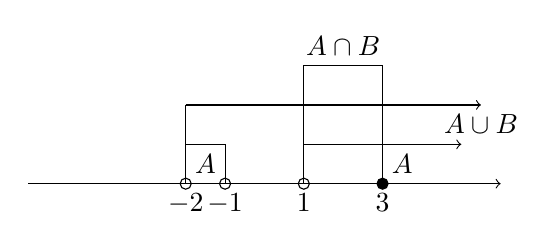
\begin{tikzpicture} [scale=0.5]
					\draw [black] [->] (-6, 0)--(6, 0);

					\draw [black] (-2, 0) circle (4pt) node[anchor=north] {$-2$};
					\draw [black] (-1, 0) circle (4pt) node[anchor=north] {$-1$};
					\draw [black] (1, 0) circle (4pt) node[anchor=north] {$1$};
					\draw [black] (-2, 0)--(-2, 1)--(-1.5, 1) node[anchor=north] {$A$};
					\draw [black] (-1.5, 1)--(-1, 1)--(-1, 0);
					\draw [black] (1, 0)--(1, 1)--(3.5, 1) node[anchor=north] {$A$};
					\draw [black] [->] (3.5, 1)--(5, 1);
					
					\draw [black] (-2, 0)--(-2, 2);
					\draw [black] [->] (-2, 2)--(5.5, 2) node[anchor=north] {$A\cup B$};

					\filldraw [black] (3, 0) circle (4pt) node[anchor=north] {$3$};

					\draw [black] (1, 0)--(1, 3)--(2, 3) node[anchor=south] {$A\cap B$};

					\draw [black] (2, 3)--(3, 3)--(3, 0);
				\end{tikzpicture}
				$$

				于是可得$B=[a, 3], a\leq 3, b=3.$

				又有$A=(-2, -1)\cup(1, +\infty), A\cap B=(1, 3]$有$[-1, 1]\subseteq B, \forall x\in (-2, -1): x\notin B.$

				于是$a=-1, b=3, B=[-1, 3].$

				\textcolor{red}{\textbf{总结:(我也不是很明白这题和补集有啥关系)(1) 涉及到区间的题目要善于使用数轴(这个真的很重要) (2) 区间的交、并、补题型中,新数往往是题目的突破口(例如本题为3).}}

		\pagebreak

		\subsection{常用逻辑用语}
			\subsubsection{命题}
				\textbf{命题}:可以判断真假的语句. 可表示为“若$\alpha$,则$\beta$”的形式,其中$\alpha$称为条件,$\beta$称为结论.

				\textbf{真命题}:含义判断为真的命题,指\textbf{所有}满足条件$\alpha$的对象都满足结论$\beta$,即$\{x|x\text{ 满足 }\alpha\}\subseteq\{x|x\text{ 满足 }\beta\}$. 考虑到$\forall x$,证明真命题需要\textbf{具体证明}.

				\textbf{假命题}:含义判断为假的命题,指\textbf{存在}满足条件$\alpha$的对象不满足结论$\beta$,即$\{x|x\text{ 满足 }\alpha\}\nsubseteq\{x|x\text{ 满足 }\beta\}$. 考虑到$\exists x$,证明假命题只需\textbf{举一反例}.

				\textbf{推出}:如果命题“若$\alpha$,则$\beta$”是真命题,那么就称$\alpha$推出$\beta$,记作$\alpha\Rightarrow\beta$或$\beta\Leftarrow\alpha$.

				\textbf{等价}:如果$\alpha\Rightarrow\beta$且$\beta\Rightarrow\alpha$,则称$\alpha$与$\beta$等价,记作$\alpha\Leftrightarrow\beta$.

				\textbf{范围与推出}:由真命题的定义,易得\textbf{$\text{小范围}\Rightarrow\text{大范围}$}.

				\textbf{传递性}:子集关系具有同向的传递性,因此推出关系也具有同向的\textbf{传递性}.

				\textbf{逆命题}:若$\alpha$,则$\beta$$\xleftrightarrow{\text{互为逆命题}}$若$\beta$,则$\alpha$. 真假没有必然联系.

				\textbf{否命题}:若$\alpha$,则$\beta$$\xleftrightarrow{\text{互为否命题}}$若$\overline{\alpha}$,则$\overline{\beta}$. 真假没有必然联系.

				\textbf{逆否命题}:若$\alpha$,则$\beta$$\xleftrightarrow{\text{互为逆否命题}}$若$\overline{\beta}$,则$\overline{\alpha}$. 同真同假,即一个命题与其逆否命题等价(逆命题与否命题互为逆否命题).

				\textbf{部分逻辑关系的反面}:是$\xleftrightarrow{\text{否}}$不是. 都是$\xleftrightarrow{\text{否}}$不都是. 至少一个$\xleftrightarrow{\text{否}}$一个也没有. 至多一个$\xleftrightarrow{\text{否}}$至少两个. 且$\xleftrightarrow{\text{否}}$或.

				~\\

				\textbf{例}:等腰$\Delta ABC$中,$AB=AC$. 已知$\angle DAP \neq \angle PAC$,求证:$AP\nparallel BC$.

				$$
				\begin{tikzpicture}[scale=0.25]
					\draw (-3, 0)--(3, 0) node [anchor=north] {$C$};
					\draw (3, 0)--(0, 10) node [anchor=east] {$A$};
					\draw (0, 10)--(-3, 0) node [anchor=north] {$B$};
					\draw (0, 10)--(6, 10) node [anchor=west] {$P$};
					\draw (0, 10)--(3, 20) node [anchor=west] {$D$};
				\end{tikzpicture}
				$$

				本题逆否命题是:等腰$\Delta ABC$中,$AB=AC$. 已知$AP\parallel BC$,则$\angle DAP = \angle PAC$.

				$\because AB=AP$

				$\therefore \angle B=\angle C$

				$\because AP\parallel BC$

				$\therefore \angle DAP=\angle B, \angle PAC=\angle C$

				$\because \angle B=\angle C$

				$\therefore \angle DAP=\angle PAC.$

				逆否命题为真命题,则原命题也为真.

				\textcolor{red}{\textbf{总结:当直接证明一个命题为真不容易时,可以利用逆否命题与原命题的等价性,证明其逆否命题为真.}}

			\subsubsection{条件}
				$$
				\begin{array}{cccc}
				&\text{$p$是$q$的}&\text{命题“若$p$,则$q$”}&P=\{x|x\text{满足性质}p\},Q=\{x|x\text{满足性质}q\}\\
				p\Rightarrow q&\text{充分条件}&\text{原命题\textbf{真}}&P\subseteq Q\\
				q\Rightarrow p&\text{必要条件}&\text{逆命题\textbf{真}}&P\supseteq Q\\
				p\Leftrightarrow q&\text{充要条件}&\text{原命题\textbf{真}且逆命题\textbf{真}}&P=Q\\
				p\Rightarrow q \textbf{ and } q\nRightarrow p&\text{充分不必要条件}&\text{原命题\textbf{真}且逆命题\textbf{假}}&P\subset Q\\
				q\Rightarrow p \textbf{ and } p\nRightarrow q&\text{必要不充分条件}&\text{原命题\textbf{假}且逆命题\textbf{真}}&P\supset Q\\
				p\nRightarrow q \textbf{ and } q\nRightarrow p&\text{既不充分也不必要条件}&\text{原命题\textbf{假}且逆命题\textbf{假}}&P\nsubseteq Q \textbf{ and } P\nsupseteq Q\\
				\end{array}
				$$

				~\\

				\textbf{例}:$P=[-2, 10], Q=\{x|1-m\leq x\leq 1+m\}(m>0).$ 若$\text{命题}\alpha: x\in P$是$\text{命题}\beta: x\in Q$的充分不必要条件,求$m$.
				~\\

				即$P\subset Q$.

				$\because m>0 \therefore m+1>1-m \therefore Q\neq \emptyset$.

				分三类讨论.

				\begin{enumerate}[label=$\arabic*^{\circ}$]
					\item $\displaystyle\left\{\begin{array}{rcl}1-m&<&-2\\1+m&>&10\end{array}\right.\Rightarrow m>9.$

					\item $1-m=-2$即$m=3$, $Q=[-2, 4]$舍.

					\item $1+m=10$即$m=9$, $Q=[-8, 10]$符合条件.
				\end{enumerate}

				综上,$m\in[9, +\infty).$

				\textcolor{red}{\textbf{总结:(1) 已知条件的充要关系,求解使用集合的子集关系求解 (2) 真子集的关系分类讨论:空集(本题的小集合为定集合,无需讨论)、两端都取不到、一端取得到带入检验.}}

			\subsubsection{反证法}

				\textbf{反证法}:通过否定结论,推出矛盾,进而证明命题成立的方法.

				~\\

				\textbf{例}:设$n\in\mathbf{Z}.$ 证明:若$n^2$是偶数,则$n$也是偶数.
				~\\

				假设结论$n$是偶数不成立,即假设$n$是奇数. 令$n=2k+1 (k\in\mathbf{Z})$,有:

				$$n^2=(2k+1)^2=4k^2+4k+1=4(k^2+k)+1,$$

				说明$n^2$是奇数,与已知条件$n^2$是偶数矛盾.

				于是假设不成立,即$n$是偶数.

				\textcolor{red}{\textbf{总结:反证法是否定结论推出矛盾,与使用逆否命题证明不同.}}

\end{document}